\lhead{\emph{Evaluation}}
\chapter{Evaluation}
% Intro
As mentioned in section TODO:ref the scope of the implementation in this thesis is limited to study the effects of exploring and navigating to music tracks. To study whether the Spatial Music Menu could compete with a touch and vision-based music player interface we designed and conducted an experiment where users should navigate to specific music tracks while using the biking simulation system described in section TODO:ref. The experiment was conducted on both types of systems.

To validate the design of the Spatial Music Menu the following hypotheses were derived for the experiment:

\begin{description}
\item[Hypthesis 1:] Replacing the input/output modalities of touch and vision with head gestures and audio (respectively) in a music player interface will increase the users ability to monitor and detect the surroundings in a biking scenario.
\end{description}

\begin{description}
\item[Hypothesis 2:] Spatial audio can provide an effective way of exploring content in form of non-speech sounds (music tracks) and combined with head gestures it can compete with a touch and vision-based interface in terms of navigation and usability.
\end{description}



% Limitations and scope
- Only 5 participants, no statistical arguments but just hints

- Possibly biased participants (friends) wants to perform good

- Limited measurement parameters e.g. not biking speed


\section{Experiment Setup}
- stationary bike, big screen, detection button, python script


\section{Method}
% Intro, overall
The user were to perform tasks while riding on a stationary bike. To simulate obstacles that the user should be aware of or respond to in a real world biking scenario, a big screen was placed in front of the user displaying circles in a random time interval. The user should detect these circles by clicking on a button attached close to the user preferred hand on the steer (in this case a Playstation 3 joystick strapped with tape).

% Task description
Artist - Album - Track\\
Task traditional: Pick phone from pocket, activate, navigate, deactivate, back in pocket

% Prerequisites
Before starting the experiment the user were instructed in how the Spatial Music Menu works i.e. which head gestures to use for navigating and how the menu structure looks. They then got a chance to try out the system both standing still and while riding the stationary bike. In the standing still scenario the user was allowed to look at the menu envisioned on the iPad screen to get a sense of the menu structure and interaction feedback. Besides trying out the Spatial Music Menu the user also got to try out a traditional music player (Deezer, TODO: ref)

\subsection{User performance}
% Number of circles, safety
The most important task for the user during testing is to detect as many circles as possible. The number of circles shown and the number of circles detected were logged during execution of tasks. This will give a quantitative analysis of whether the user is able to monitor the surroundings while interacting with the systems and contribute to the safety problem focus.

% System, track exploring
For measuring the content (music track) exploring part of the Spatial Music Menu all navigation information were logged on the iPad. 

% System, task time


\subsection{Measuring workload}
Subjective workload was measured using the NASA Task Load Index (TLX) scales \cite{hart_workload_1990}. The scales includes mental demand, physical demand, temporal demand, performance, effort and frustration in which each participant should rate after testing (for both the Spatial Music Menu and the touch and vision-based music player). 

The user ratings gives a qualitative analysis of the system and the perceived workload is linked with the general usability of the system. It can give an indication of how much of the users physical and mental resources is required by the system during interaction and thereby an indication of the resources left for monitoring and navigating the surroundings when biking i.e. a safety parameter.


\section{Participants}
5 persons (all male) were chosen for the evaluation. They all have in common that they listens to music while biking regurarly. The participants had an average age of 30 years.


\section{Results}
...

\subsection{User performance}
...

Circles detected, figure \ref{fig:resultscircles}

\begin{figure}[htbp]
	\centering
		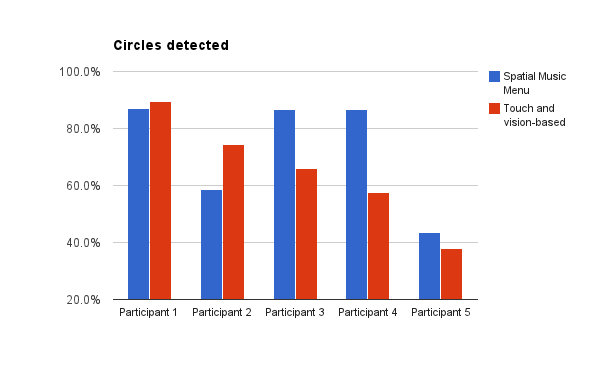
\includegraphics[width=0.9\textwidth,height=\textheight,keepaspectratio]{./Figures/results_circles.png}
		\rule{35em}{1pt}
	\caption[Results circle detections]{Percentage of circles detected for the participants}
	\label{fig:resultscircles}
\end{figure}


Task time execution, figure \ref{fig:resultstasktime}

\begin{figure}[htbp]
	\centering
		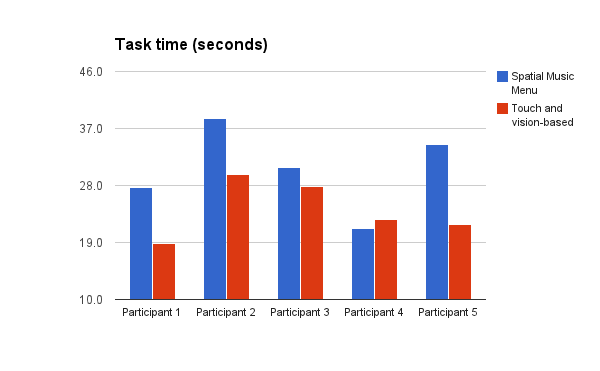
\includegraphics[width=0.9\textwidth,height=\textheight,keepaspectratio]{./Figures/results_task_time.png}
		\rule{35em}{1pt}
	\caption[Results task time]{Time taken (in seconds) in average to execute a task for the participants}
	\label{fig:resultstasktime}
\end{figure}

\subsection{Workload}
...

Nasa TLX scores, figure \ref{fig:resultsnasatlx}

\begin{figure}[htbp]
	\centering
		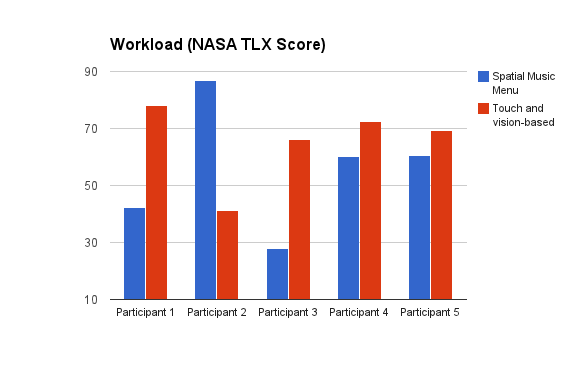
\includegraphics[width=0.9\textwidth,height=\textheight,keepaspectratio]{./Figures/results_nasatlx.png}
		\rule{35em}{1pt}
	\caption[Results NASA TLX Score]{NASA TLX overall workload score for the participants (less is better)}
	\label{fig:resultsnasatlx}
\end{figure}

\subsection{Discussion}
...


%Track:\\
%Quadratic track marked with cones including a cone in the middle on every side for the user to navigate around (track 50x50m)

%User/device setup:\\
%1. User head gestures setup and tracks setup\\
%2. User demoing both systems while standing still (practice)\\
%3. User demoing both systems while biking (practice)

%Round:\\
%1. Before start user get task - a track in which he/she should navigate to\\
%2. User starts biking - when sign given (whistle), the user should perform the task\\
%3. When task is finished the user raises a hand and stops\\
%4. Step 1-3 is repeated 5 times\\
%5. This evaluation is performed with both traditional and prototype system (3 times for each)

%Measurements:\\
%1. Time taken to complete a task (every task is noted on paper)\\
%2. Distance in total for 1 round\\
%3. Prototype system logging of activities (e.g. menu state switch, device connection state, gestures recognized)

%Results linked to problem statement:\\
%1. [Efficiency] Time and distance comparison between traditional and prototype system\\
%2. [Learnability] Comparison/progress between 1. round and 3. round with new prototype system\\
%3. [Usability (cognitive load)] Users answering questions (form)\\
%4. [Suitability to real-world hands- and eyes occupied situations] Summary of 1-3 above







% Iterations, measurable comparison between new system and traditional

% 2 evaluations - closed lab (1 day) and open (real life, week(s))

% Idea for closed lab exercise - Multiple lists of songs. A user shouls navigate and play the different songs with head gestures and normal navigation. Compare these in relation to time taken, cognitive load (eyes and at least one hand occupied), user feel of frustration (cognitive load) when navigating

% Final evaluation:
% Idea: Time to find a song, level of frustration (cognitive load) for finding song

% NB: For final evaluation - device with 3G+ connection and added to apple developer team, should be executed latest mid of April so finished end of April (1/2 weeks trial), 2 testpersons -> 1 experienced tech person and 1 non-tech/average user


% Maybe comfort as a measurement?
%(Taken from Brewster article)
%The final measure taken was comfort. This was based around a new scale developed by Knight et al. [10] called the Comfort Rating Scale (CRS) which assesses various aspects to do with the comfort of a wearable device. For a device to be accepted and used it needs to be comfortable and people need to be happy to wear it. Using a range of 20- point rating scales similar to NASA TLX, CRS breaks com- fort into 6 categories: emotion, attachment, harm, perceived change, movement and anxiety. Knight et al. have used it to assess the comfort of two wearable devices they are building in their research group. Using this will allow us to find out more about the actual acceptability our systems.